A square piece of paper has sides of length $ 100$. From each corner a wedge is cut in the following manner: at each corner, the two cuts for the wedge each start at distance $ \sqrt {17}$ from the corner, and they meet on the diagonal at an angle of $ 60^\circ$ (see the figure below). The paper is then folded up along the lines joining the vertices of adjacent cuts. When the two edges of a cut meet, they are taped together. The result is a paper tray whose sides are not at right angles to the base. The height of the tray, that is, the perpendicular distance between the plane of the base and the plane formed by the upper edges, can be written in the form $ \sqrt [n]{m}$, where $ m$ and $ n$ are positive integers, $ m < 1000$, and $ m$ is not divisible by the $ n$th power of any prime. Find $ m + n$.

\begin{center}
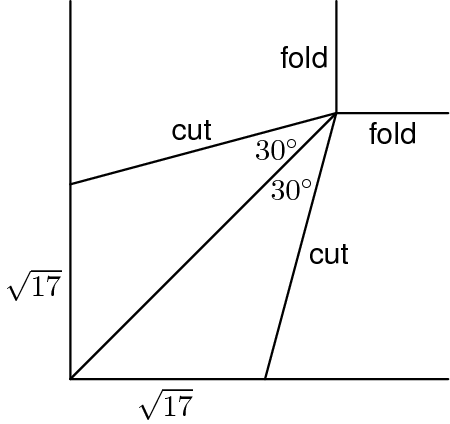
\includegraphics[width = 45.0mm]{img/fig0.png}
\end{center}